\documentclass[11pt,a4paper]{article}
\usepackage[margin=2.3cm]{geometry}
\IfFileExists{lmodern.sty}{\usepackage{lmodern}}{}
\usepackage[T1]{fontenc}
\usepackage{titlesec,tabularx,longtable,booktabs,array,enumitem,xcolor,fancyhdr,amsmath}
\usepackage{listings}
\usepackage{tikz}
\usetikzlibrary{arrows.meta,positioning,fit,calc,shapes.geometric,backgrounds}
\usepackage[hyphens]{url}
\usepackage{hyperref}

\definecolor{headcolor}{RGB}{15,70,60}
\definecolor{boxa}{RGB}{226,239,236}
\definecolor{boxb}{RGB}{238,242,250}
\definecolor{boxc}{RGB}{250,243,230}
\definecolor{boxd}{RGB}{245,245,245}
\definecolor{edge}{RGB}{70,70,70}
\hypersetup{colorlinks=true,linkcolor=headcolor,urlcolor=headcolor,
  pdftitle={TrustBazaar System Design - Unit 5: Game-Account Escrow},
  pdfauthor={S. M. Nihal Ahmed, Afrim Hossen Khan, Sabikun Nahar Sinthia}}

\titleformat{\section}{\normalfont\Large\bfseries\color{headcolor}}{\thesection}{10pt}{}
\titleformat{\subsection}{\normalfont\large\bfseries}{\thesubsection}{8pt}{}
\titleformat{\subsubsection}{\normalfont\normalsize\bfseries}{\thesubsubsection}{6pt}{}
\pagestyle{fancy}\fancyhf{}
\fancyhead[L]{System Design Document}\fancyhead[R]{Unit 5: Game-Account Escrow}
\fancyfoot[C]{\thepage}\renewcommand{\headrulewidth}{0.4pt}\setlength{\headheight}{14pt}
\setlength{\emergencystretch}{3em}
\setlength{\parskip}{0.45em}\setlength{\parindent}{0pt}

\lstdefinelanguage{SQLpg}{morekeywords={CREATE,TABLE,TYPE,AS,ENUM,PRIMARY,KEY,REFERENCES,NOT,NULL,DEFAULT,CHECK,UNIQUE,INDEX,ON,WHERE,TRIGGER,BEFORE,INSERT,UPDATE,DELETE,FOR,EACH,ROW,EXECUTE,FUNCTION,RETURNS,LANGUAGE,BEGIN,END,IF,THEN,ELSE,RETURN,SELECT,FROM,INTO,ORDER,BY,DESC,LIMIT,GRANT,REVOKE,TO,SCHEMA,EXTENSION,EXISTS,OR,AND,IN,IS,ALTER,ADD,FOREIGN,GENERATED,ALWAYS,IDENTITY,DEFERRABLE,INITIALLY,DEFERRED,DECLARE,PERFORM,LOOP,RAISE,EXCEPTION,USING,DISTINCT,ROLE,LOGIN,USAGE,ALL,TABLES,STABLE,DO},sensitive=false,morecomment=[l]{--},morestring=[b]'}
\lstdefinelanguage{JS}{morekeywords={import,export,from,const,let,async,await,function,return,new,if,throw,try,catch,for,of,true,false,null},sensitive=true,morecomment=[l]{//},morestring=[b]",morestring=[b]`}
\lstset{basicstyle=\ttfamily\scriptsize,columns=fullflexible,keepspaces=true,breaklines=true,
  keywordstyle=\color{headcolor}\bfseries,commentstyle=\color{gray}\itshape,frame=single,rulecolor=\color{gray!40},
  upquote=true,literate={–}{{--}}1}

\newenvironment{dtable}[1]{\small\begin{longtable}{#1}}{\end{longtable}}

\begin{document}
\begin{titlepage}
\centering
\vspace*{1cm}
{\Large Daffodil International University}\\[0.2cm]
{\large Department of Software Engineering}\\[2cm]
\rule{\linewidth}{0.5pt}\\[0.4cm]
{\huge\bfseries System Design Document}\\[0.3cm]
{\LARGE Unit 5: Game-Account Escrow}\\[0.3cm]
{\large TrustBazaar: A Verified Peer-to-Peer Auction and Marketplace Platform for Used Goods}\\[0.2cm]
\rule{\linewidth}{0.5pt}\\[1.6cm]
{\large S. M. Nihal Ahmed (232-35-002)\\[0.1cm] Afrim Hossen Khan (232-35-076)\\[0.1cm] Sabikun Nahar Sinthia (232-35-475)}\\[1.6cm]
\begin{tabular}{|l|>{\raggedright\arraybackslash}p{8cm}|}
\hline
\textbf{Status} & Draft for team review \\ \hline
\textbf{Version} & 0.1, 18 October 2026 \\ \hline
\textbf{Implements} & SRS v2.0 (\texttt{docs/srs.tex}) \\ \hline
\textbf{Depends on} & Unit 1 (Identity \& Access), Unit 2 (Order, Payment \& Escrow), Unit 3 (Auctions, Listings \& Search); Unit 4 not used \\ \hline
\textbf{Database schema} & \texttt{docs/design/sql/05\_game\_accounts.sql}, tested on PostgreSQL (70 checks, concurrency tests) and the browser code in Chromium (14 checks); Appendix B \\ \hline
\end{tabular}
\vfill
\end{titlepage}
\tableofcontents
\newpage
\section{Introduction}

\subsection{Purpose}
This document is the fifth unit of TrustBazaar's System Design Document. It covers what a game account needs in place of physical delivery:
\begin{itemize}[nosep]
  \item \textbf{proof of ownership} before the listing is published;
  \item \textbf{a sealed credential handover}: the seller's browser encrypts the login details with a key that only the buyer's browser holds, so the platform stores them but can never read them;
  \item \textbf{a guided takeover}, whose completion is the order's delivery event;
  \item \textbf{a protection period}, during which the payment stays in escrow in case the seller recovers the account.
\end{itemize}
The unit's central claim is security objective 2 of the SRS: \emph{the server and its staff never hold game-account credentials in readable form} (SEC-GAM-01). This document shows how that is achieved and tested, and states plainly where the protection stops (SRS assumption AS-6).

The unit follows conventions DC-1 to DC-14 (Units 1, 2 and 4). It uses Unit~2's escrow through \texttt{EscrowCommands}, approves listings through Unit~3's \texttt{ListingsCommands}, and does not use Unit~4: game accounts have no delivery (FR-GAM-06).

\subsection{Scope}
\textbf{In scope:}
\begin{itemize}[nosep]
  \item the games catalogue and the structured game fields of a listing;
  \item ownership codes, proof screenshots, their review, and one live listing per player ID;
  \item the publisher-risk disclosure and its acknowledgement;
  \item the buyer's key pair, the fingerprint, the sealing and opening of credentials in the browser, and the credential-access log;
  \item the takeover checklist, the takeover window, re-keying, \texttt{credentials\_invalid} reports, and deletion of the ciphertext;
  \item the evidence needed when a seller recovers a sold account (FR-GAM-18);
  \item the feature switch CP-36.
\end{itemize}

\textbf{Out of scope, owned by other units:}
\begin{itemize}[nosep]
  \item the protection period's escrow hold, early release and the payout (Unit~2, release policy \texttt{game\_protection});
  \item the listing itself, its price, photos and visibility (Unit~3);
  \item notifications and the chat warning of FR-GAM-20 (Unit~6);
  \item disputes, the ownership-proof queue screens, suspension, blacklisting and the evidence export (Unit~7, with Unit~1's approvals);
  \item the screens themselves (Unit~8); this document fixes what they must do and supplies the browser code they use.
\end{itemize}

\subsection{Requirements covered}
\begin{itemize}[nosep]
  \item \textbf{Functional:} FR-GAM-01 to FR-GAM-20; FR-PAY-07 and FR-PAY-08 (game side); FR-DSP-01 (game windows); FR-DSP-05 (game evidence); FR-NTF-07 and FR-NTF-08 (deadlines; nothing secret in notifications).
  \item \textbf{Security:} SEC-GAM-01 to SEC-GAM-03; SEC-DAT-07, SEC-DAT-10; SEC-AUTH-08 (step-up for early release, applied by Unit~2); SEC-IRM-04 (switching the feature off).
  \item \textbf{Other:} IF-UI-06, IF-SW-07; NFR-USE-03; NFR-MNT-02 (game-account release rules); DR-07; AS-5, AS-6.
\end{itemize}

% ------------------------------------------------------------------
\section{Unit Overview}

\subsection{Responsibilities}
\begin{enumerate}[nosep]
  \item Publish a game-account listing only after an operator has checked a fresh ownership code on the seller's game profile, and never let two live listings claim the same player ID.
  \item Get the login details from the seller's browser to the buyer's browser without the platform ever being able to read them.
  \item Record exactly one fulfilment step (first credential delivery) and one delivery event (takeover complete) for Unit~2's escrow, at the right moments.
  \item Keep a complete, append-only record of who retrieved the sealed credentials and which takeover steps the buyer confirmed, for disputes and, if needed, for a complaint to law enforcement.
  \item Delete the ciphertext as soon as the order is over.
\end{enumerate}

\subsection{Who can see what}
\label{sec:boundary}
\begin{figure}[!htbp]
\centering
\resizebox{\textwidth}{!}{%
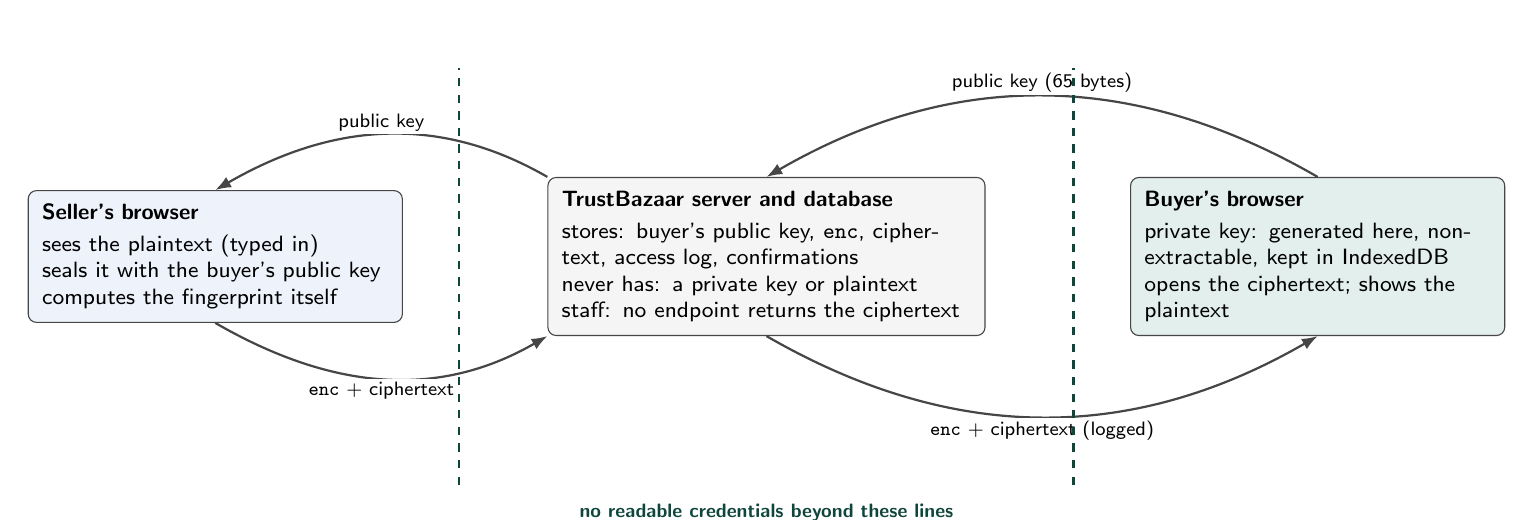
\begin{tikzpicture}[font=\sffamily\footnotesize,
  box/.style={draw=edge, rounded corners=3pt, align=left, inner sep=5pt, text width=4.4cm},
  arr/.style={-{Latex[length=2mm]}, draw=edge, thick},
  lb/.style={font=\sffamily\scriptsize, align=center, fill=white, inner sep=1pt}]
\node[box, fill=boxb] (s) at (0,0) {\textbf{Seller's browser}\\[2pt] sees the plaintext (typed in)\\ seals it with the buyer's public key\\ computes the fingerprint itself};
\node[box, fill=boxd, text width=5.2cm] (srv) at (7.0,0) {\textbf{TrustBazaar server and database}\\[2pt] stores: buyer's public key, \texttt{enc}, ciphertext, access log, confirmations\\ never has: a private key or plaintext\\ staff: no endpoint returns the ciphertext};
\node[box, fill=boxa] (b) at (14.0,0) {\textbf{Buyer's browser}\\[2pt] private key: generated here, non-extractable, kept in IndexedDB\\ opens the ciphertext; shows the plaintext};
\draw[arr] (b.north) to[out=150, in=30] node[lb, above]{public key (65 bytes)} (srv.north);
\draw[arr] (srv.north west) to[out=150, in=30] node[lb, above]{public key} (s.north);
\draw[arr] (s.south) to[out=-30, in=-150] node[lb, below]{\texttt{enc} + ciphertext} (srv.south west);
\draw[arr] (srv.south) to[out=-30, in=-150] node[lb, below]{\texttt{enc} + ciphertext (logged)} (b.south);
\draw[dashed, draw=headcolor, thick] (3.1,-2.9) -- (3.1,2.4);
\draw[dashed, draw=headcolor, thick] (10.9,-2.9) -- (10.9,2.4);
\node[font=\sffamily\scriptsize\bfseries, text=headcolor] at (7.0,-3.25) {no readable credentials beyond these lines};
\end{tikzpicture}}
\caption{Trust boundary of the sealed handover. The server relays and stores only what it cannot decrypt (SEC-GAM-01). AS-6: this assumes the code the server sends to the browsers has not been altered.}
\label{fig:boundary}
\end{figure}

\subsection{Components}
\begin{dtable}{@{}>{\raggedright\arraybackslash}p{4.1cm}>{\raggedright\arraybackslash}p{11.1cm}@{}}
\toprule
\textbf{Component} & \textbf{Responsibility} \\ \midrule \endhead
\multicolumn{2}{@{}l}{\textit{Backend module \texttt{game-accounts}}} \\
GameListingService & Game fields; issues ownership codes; receives proof screenshots; refuses listings while CP-36 is off (Section~\ref{sec:listing}). \\
OwnershipReviewService & Operator review of proofs; takes the player-ID claim; asks Unit~3 to publish (Section~\ref{sec:review}). \\
HandoverService & Disclosure, buyer key, credential delivery and retrieval, re-key, reports; the DC-14 calls to \texttt{EscrowCommands} (Section~\ref{sec:sealed}). \\
TakeoverService & Checklist confirmations and completion (Section~\ref{sec:takeover}). \\
GameJobs & Window-end completion, re-key overdue, proof expiry (Section~\ref{sec:jobs}). \\
EvidenceService & Assembles the evidence for disputes and for FR-GAM-18. \\
\multicolumn{2}{@{}l}{\textit{Browser module \texttt{sealed.js} (Appendix~\ref{app:js}), used by the Unit~8 screens}} \\
Key manager & Generates the buyer's non-extractable key pair and keeps it in IndexedDB. \\
Sealer / opener & HPKE seal in the seller's browser, open in the buyer's; padding; the fingerprint. \\
\bottomrule
\end{dtable}
\section{Interfaces}

\subsection{HTTP API}
\label{sec:api}
All paths are under \texttt{/api/v1}; policies and rate limits are those of Unit~1. Binary values travel as base64url. Responses that carry a public key or a ciphertext are sent with \texttt{Cache-Control: no-store}, and no response ever carries a fingerprint (Section~\ref{sec:fingerprint}).

{\small
\begin{longtable}{@{}>{\ttfamily\raggedright\arraybackslash}p{1.55cm}>{\ttfamily\raggedright\arraybackslash}p{4.8cm}>{\raggedright\arraybackslash}p{2.4cm}>{\raggedright\arraybackslash}p{6.1cm}@{}}
\toprule
\textnormal{\textbf{Method}} & \textnormal{\textbf{Path}} & \textbf{Policy} & \textbf{Purpose (requirement)} \\ \midrule \endhead
\multicolumn{4}{@{}l}{\textbf{Listing a game account}} \\
GET & /\allowbreak games & Public & Games, platforms, where the code goes, the publisher note \\
PUT & /\allowbreak listings/\allowbreak \{id\}/\allowbreak game-\allowbreak details & Verified(list), seller & Game, platform, player ID, contents (FR-GAM-02) \\
POST & /\allowbreak listings/\allowbreak \{id\}/\allowbreak ownership-\allowbreak code & Seller & Issue a code valid for DV-33 (FR-GAM-03) \\
POST & /\allowbreak listings/\allowbreak \{id\}/\allowbreak ownership-\allowbreak proof & Seller & Upload the screenshot; submits the proof \\
\multicolumn{4}{@{}l}{\textbf{Checkout} (before payment)} \\
POST & /\allowbreak orders/\allowbreak \{id\}/\allowbreak game/\allowbreak acknowledge & Buyer & Accept the disclosure, by version (FR-GAM-05) \\
POST & /\allowbreak orders/\allowbreak \{id\}/\allowbreak game/\allowbreak key & Buyer & Register the browser's public key (FR-GAM-07) \\
\multicolumn{4}{@{}l}{\textbf{Handover and takeover} (after payment)} \\
GET & /\allowbreak orders/\allowbreak \{id\}/\allowbreak game & Buyer or seller & Status, deadlines, countdowns, confirmed steps (NFR-USE-03) \\
GET & /\allowbreak orders/\allowbreak \{id\}/\allowbreak game/\allowbreak buyer-\allowbreak key & Seller & The buyer's current public key and its version \\
POST & /\allowbreak orders/\allowbreak \{id\}/\allowbreak game/\allowbreak sealed & Seller & Deliver \texttt{enc} and ciphertext for that version (FR-GAM-09, 10) \\
GET & /\allowbreak orders/\allowbreak \{id\}/\allowbreak game/\allowbreak sealed & Buyer & Retrieve them; every call is logged (FR-GAM-11) \\
POST & /\allowbreak orders/\allowbreak \{id\}/\allowbreak game/\allowbreak takeover-\allowbreak steps/\allowbreak \{step\} & Buyer & Confirm a checklist step (FR-GAM-13) \\
POST & /\allowbreak orders/\allowbreak \{id\}/\allowbreak game/\allowbreak report-\allowbreak invalid & Buyer & ``The credentials do not work'': opens a dispute (FR-GAM-14) \\
POST & /\allowbreak orders/\allowbreak \{id\}/\allowbreak game/\allowbreak rekey & Buyer & New public key after losing the old one (FR-GAM-12) \\
POST & /\allowbreak orders/\allowbreak \{id\}/\allowbreak release-\allowbreak early & Buyer, StepUp & Unit~2's endpoint (FR-GAM-17, SEC-AUTH-08) \\
\multicolumn{4}{@{}l}{\textbf{Staff}} \\
GET & /\allowbreak staff/\allowbreak game/\allowbreak ownership-\allowbreak proofs & Staff(operator) & The proof queue (FR-OPS-01) \\
GET & /\allowbreak staff/\allowbreak game/\allowbreak ownership-\allowbreak proofs/\allowbreak \{id\}/\allowbreak screenshot & Staff(operator) & Signed link valid CP-31; each view audited \\
POST & /\allowbreak staff/\allowbreak game/\allowbreak ownership-\allowbreak proofs/\allowbreak \{id\}/\allowbreak review & Staff(operator) & Approve, or reject with a reason, recording the live-profile check \\
POST, PATCH & /\allowbreak admin/\allowbreak games & Staff(admin) & Maintain the games catalogue \\
\bottomrule
\end{longtable}
}

There is deliberately no staff endpoint that returns a ciphertext or a public key, and the evidence for a case (Section~\ref{sec:evidence}) contains neither. Refusals return \texttt{422} with a stable code, among them \texttt{feature\_off}, \texttt{player\_id\_claimed}, \texttt{code\_expired}, \texttt{key\_fixed}, \texttt{stale\_key\_version}, \texttt{deadline\_passed}, \texttt{window\_ended}, \texttt{recovery\_email\_confirmed} and \texttt{rekey\_used}.

\subsection{Ports provided}
\begin{lstlisting}[language=Java,morekeywords={interface,type,Promise,string,boolean,number,bigint}]
interface GameAccountPort {                       // used by Unit 2
  assertCheckoutReady(orderId: string): Promise<void>;   // disclosure acknowledged, key registered, CP-36 on
}
interface GameAccountCommands {                   // used by Unit 7
  reviewProof(proofId: string, staffId: string, approve: boolean,
              liveCheck: 'matched' | 'not_matched' | 'not_available', reason?: string): Promise<void>;
  disputeWithdrawn(orderId: string, tx: EntityManager): Promise<void>;
}
interface GameAccountQueries {                    // used by Units 6 and 7
  evidence(orderId: string): Promise<GameEvidence>;           // FR-DSP-05, FR-GAM-18
  credentialsInvalidAllowed(orderId: string): Promise<boolean>;  // FR-GAM-14
  deadlines(orderId: string): Promise<GameDeadlines>;         // for reminders (FR-NTF-07)
}
\end{lstlisting}

\subsection{Events}
\begin{dtable}{@{}>{\raggedright\arraybackslash}p{6.4cm}>{\raggedright\arraybackslash}p{8.8cm}@{}}
\toprule
\textbf{Event} & \textbf{Use} \\ \midrule \endhead
\multicolumn{2}{@{}l}{\textit{Published (outbox, DC-6). No payload ever contains key material or ciphertext.}} \\
\texttt{game\_accounts.\allowbreak ownership.approved}, \texttt{.rejected} & Unit~3 publishes or returns the listing; notifications. \\
\texttt{game\_accounts.\allowbreak credentials.requested} & Notifications to the seller, with the CP-22 deadline. \\
\texttt{game\_accounts.\allowbreak credentials.delivered} & Notifications to the buyer, with the takeover deadline. \\
\texttt{game\_accounts.\allowbreak credentials.\allowbreak reported\_invalid} & Disputes (opened in the same transaction); notifications. \\
\texttt{game\_accounts.\allowbreak rekey.requested}, \texttt{.overdue} & Notifications to the seller; Disputes when overdue. \\
\texttt{game\_accounts.\allowbreak takeover.completed} & Notifications: the protection period's end date. The escrow change is made in the same transaction (DC-14). \\
\multicolumn{2}{@{}l}{\textit{Consumed (idempotent)}} \\
\texttt{orders.order.paid} (game account) & \texttt{mark\_paid}: ask the seller for the credentials, with the order's CP-22 deadline (FR-GAM-10). \\
\texttt{orders.escrow.refunded} before the delivery event & \texttt{finish(before)}: handover cancelled, ciphertext deleted. \\
\texttt{orders.escrow.released}, \texttt{.refunded}, \texttt{.partially\_refunded} after it & \texttt{finish(after)}: handover closed, ciphertext deleted, player-ID claim released (FR-GAM-19, FR-GAM-04). \\
\texttt{listings.listing.ended\_unsold}, \texttt{.cancelled}, \texttt{.removed} & Release the claim of an unsold listing. \\
\bottomrule
\end{dtable}

\subsection{Ports required}
\begin{dtable}{@{}>{\raggedright\arraybackslash}p{4.6cm}>{\raggedright\arraybackslash}p{10.6cm}@{}}
\toprule
\textbf{Port} & \textbf{Provider and use} \\ \midrule \endhead
\texttt{IdentityQuery}, \texttt{AuditService}, \texttt{FileVault} (Unit 1) & \texttt{assertCanTransact}; audit of reviews and screenshot views; encrypted storage of proof screenshots under a new purpose (I-31). \\
\texttt{OrdersPort}, \texttt{EscrowCommands} (Unit 2) & \texttt{lockForFulfilment} (DC-14); \texttt{recordFulfilmentStep(credentials\_delivered)}; \texttt{recordDeliveryEvent(game\_takeover, at)}. \\
\texttt{ListingsCommands} (Unit 3) & \texttt{approveForPublication} and \texttt{returnToDraft} after a review. \\
\texttt{DisputeCommands} (Unit 7) & Open a \texttt{credentials\_invalid} dispute in the same transaction as the report. \\
\texttt{ConfigPort}, \texttt{Clock} & CP-22, CP-23, CP-24, CP-36 and the DV values. \\
\bottomrule
\end{dtable}
\section{Data Design}
\label{sec:data}
The schema is in \texttt{docs/design/sql/05\_game\_accounts.sql} (Appendix~\ref{app:ddl}), loaded after Units~1 to~4. The unit owns the schema \texttt{game\_accounts}. Its foreign keys point to users, staff and sessions (Unit~1), orders (Unit~2) and listings (Unit~3), as DC-5 allows.

\tikzset{
  ent/.style={draw=edge, fill=white, rounded corners=1.5pt, align=left, inner sep=3pt, font=\sffamily\scriptsize, text width=3.9cm},
  fk/.style={-{Latex[length=1.6mm]}, draw=edge!80, semithick},
}
\newcommand{\ent}[2]{\textbf{\color{headcolor}#1}\\[-1pt]{\ttfamily\tiny #2}}
\begin{figure}[!htbp]
\centering
\resizebox{0.98\textwidth}{!}{%
\begin{tikzpicture}
\node[ent, fill=boxd] (lst) at (0,6.6) {\ent{listings.listings}{(Unit 3)}};
\node[ent, fill=boxd] (ord) at (10.4,6.6) {\ent{orders.orders}{(Unit 2)}};
\node[ent] (g) at (5.2,6.6) {\ent{games}{slug, name, platforms\\code\_placement, publisher\_note}};
\node[ent, fill=boxb] (d) at (0,4.2) {\ent{details}{listing\_id PK, seller, game\\platform, player\_id\\player\_id\_norm (generated)\\contents}};
\node[ent] (p) at (0,1.4) {\ent{ownership\_proofs}{code TB-XXXX-XXXX, expires\_at\\screenshot (encrypted file)\\status, reviewed\_by, live\_check\\one open per listing}};
\node[ent] (c) at (5.2,4.2) {\ent{claims}{game, player\_id\_norm\\listing, order, released\_at\\one live per player ID}};
\node[ent, fill=boxa, text width=4.4cm] (h) at (10.4,4.0) {\ent{handovers}{order\_id PK, listing, buyer, seller\\status, disclosure version / ack\\key\_version, rekeys\_used\\credentials\_due\_at (CP-22)\\delivered\_at, takeover\_due\_at\\five step times; taken\_over\_at\\takeover\_source}};
\node[ent] (k) at (15.6,6.0) {\ent{buyer\_keys}{(order, version) PK\\public\_key (65 bytes)\\session (append-only)}};
\node[ent, fill=boxc] (sc) at (15.6,3.7) {\ent{sealed\_credentials}{(order, key\_version) PK\\enc, ciphertext (512k+16)\\deleted\_at (only change)}};
\node[ent] (al) at (15.6,1.5) {\ent{access\_log}{order, user, session\\key\_version, ip, at\\(append-only)}};
\node[ent] (cf) at (10.4,0.9) {\ent{confirmations}{(order, step) PK\\session, at (append-only)}};
\draw[fk] (d.north) -- (lst.south);
\draw[fk] (d.north east) -- ++(0.3,0) |- (g.west);
\draw[fk] (p.north) -- (d.south);
\draw[fk] (c.west) -- (d.east|-c.west);
\draw[fk] (h.north) -- (ord.south);
\draw[fk] (h.west) -- ++(-0.6,0) |- ([yshift=-10pt]c.east);
\draw[fk] (k.west) -- ++(-0.3,0) |- ([yshift=12pt]h.east);
\draw[fk] (sc.north) -- (k.south);
\draw[fk] (al.west) -- ++(-0.3,0) |- ([yshift=-14pt]h.east);
\draw[fk] (cf.north) -- (h.south);
\end{tikzpicture}}
\caption{The \texttt{game\_accounts} schema. Handovers also reference the listing's \texttt{details}; claims reference the order once sold. Those arrows are omitted.}
\label{fig:er}
\end{figure}

\subsection{Tables and rules the database enforces}
\begin{dtable}{@{}>{\ttfamily\raggedright\arraybackslash}p{3.5cm}>{\raggedright\arraybackslash}p{11.7cm}@{}}
\toprule
\textnormal{\textbf{Table}} & \textbf{Rules enforced by the database} \\ \midrule \endhead
games & Slug format; at least one platform. \\
details & The platform must be one the game offers. Player ID printable, at least 2 characters, compared without spaces or case. Game and player ID fixed once a proof is submitted. \\
ownership\_proofs & Code format (DV-33), unique. One open proof per listing. Only the permitted status changes. Submitting needs the screenshot. A review records the operator, the time and the live-profile check; a rejection needs a reason; approval is impossible if the live profile did not match, or after the code has expired. A reviewed proof is final. \\
claims & One live claim per game and player ID (FR-GAM-04), taken only by an approval. \\
handovers & Starts as \texttt{preparing} without a key. Parties and disclosure fixed. Only the permitted status changes; cancelled and closed are final. A paid handover has a key and the CP-22 deadline. Status fields consistent. Key version $=$ re-keys $+$ 1, at most one re-key. Confirmed steps and the takeover time can never change. A checklist completion needs all five steps. A cancellation is impossible after the takeover. A closed or cancelled handover can have no ciphertext left (trigger). \\
buyer\_keys & Uncompressed P-256 point (65 bytes, \texttt{0x04}); append-only. \\
sealed\_credentials & For an existing key version. \texttt{enc} is a P-256 point; ciphertext is 512$k$ $+$ 16 bytes, at most 4~KB of plaintext. The only change ever allowed is deletion of the content. \\
access\_log, confirmations & Append-only; one confirmation per step. \\
\bottomrule
\end{dtable}

% ------------------------------------------------------------------
\section{Listing a Game Account}
\label{sec:listing}

\subsection{Details}
The seller creates the listing in Unit~3 as usual (title, description, price, fixed price or auction) and adds the game fields here: the game from the catalogue, the platform, the in-game player ID and a description of the account's contents (FR-GAM-02). The form never asks for any login detail, and Unit~3's screening terms include common words for passwords in Bangla and English, so a seller who types one into the description is held for review. While CP-36 is off, game-account listings and purchases are refused, and active ones are hidden; paid orders continue (FR-GAM-01). The switch is changed through Unit~1's administrator controls with four-eyes approval (SEC-IRM-04).

\subsection{Ownership proof}
\label{sec:review}
\begin{enumerate}[nosep]
  \item The seller asks for a code. It looks like \texttt{TB-7K4Q-9XWM}: 40 random bits in Crockford base32, without the easily confused letters I, L, O and U, valid for DV-33 (7~days). The code is not a secret; it proves that the seller controls the profile \emph{now}.
  \item The seller puts the code where the catalogue says (for example the profile signature) and uploads a screenshot showing the code and the player ID. The screenshot is Confidential, so it goes through Unit~1's \texttt{FileVault}: re-encoded without metadata, encrypted with its own data key, stored on a private volume, and shown to operators only through a signed link valid for CP-31 (each view audited).
  \item An operator compares the screenshot with the listing and, where the game has public profiles, opens the live profile and looks for the code. The result is recorded as \texttt{matched}, \texttt{not\_matched} or \texttt{not\_available}. A screenshot alone can be faked, so a mismatch on the live profile makes approval impossible (database constraint).
  \item Approval takes the player-ID claim and asks Unit~3 to publish. Rejection needs a reason, which the seller sees.
\end{enumerate}

\subsection{One live listing per player ID}
FR-GAM-04 allows at most one active listing per game and player ID, and none while an earlier sale is still in its takeover window or protection period. Both are met by one rule: a \emph{claim} on the player ID, unique while live.
\begin{itemize}[nosep]
  \item The claim is taken \emph{when ownership is approved}, not when a draft is written. Otherwise anyone could block another person's player ID by drafting a listing for it.
  \item It is released when the listing ends unsold, is cancelled or is removed, or, after a sale, when the order's escrow reaches a terminal state, which for a game account is after the protection period.
  \item Player IDs are compared without spaces and case, so \texttt{5123 4567} and \texttt{51234567} are the same.
\end{itemize}
Tested: ten operators approving ten listings of the same player ID at the same moment produced exactly one approval and one live claim.
\section{The Sealed Handover}
\label{sec:sealed}

\subsection{Choice of construction}
SEC-DAT-10 allows two options: RSA-OAEP with SHA-256 and a key of at least 3072 bits, or ECDH on P-256 with AES-256-GCM. RSA-OAEP can encrypt at most $384 - 2 \times 32 - 2 = 318$ bytes with a 3072-bit key, which a login, a long password and a set of recovery codes can exceed. The design therefore uses the ECDH option, in its standard form: \textbf{HPKE} (Hybrid Public Key Encryption, RFC~9180) in base mode, with the suite DHKEM(P-256, HKDF-SHA256), HKDF-SHA256 and AES-256-GCM (DV-35).

HPKE is the IETF's standard way of combining ECDH, a key-derivation function and AES-GCM. Using it means no construction of our own (C-4). It is implemented by the library \texttt{@hpke/core} (version 1.9.0), which is built only on the browser's Web Cryptography API (IF-SW-07). The team's own code is the thin module \texttt{sealed.js} in Appendix~\ref{app:js}. Each sealing uses a fresh ephemeral key, whose public half is sent as \texttt{enc} with the ciphertext. Two values bind a ciphertext to its context:
\begin{itemize}[nosep]
  \item the HPKE \emph{info} string \texttt{TrustBazaar/game-credentials/v1};
  \item the AES-GCM \emph{associated data} \texttt{order:<order id>|key:<key version>}, so a ciphertext copied to another order, or replayed under another key version, fails to open (tested).
\end{itemize}

\subsection{The buyer's key}
At checkout, after accepting the disclosure (FR-GAM-05), the buyer's browser:
\begin{enumerate}[nosep]
  \item checks that the Web Cryptography API and IndexedDB are available, and otherwise explains that this browser cannot take part in a game-account sale (AS-5);
  \item generates a P-256 key pair with \texttt{extractable = false} (FR-GAM-07). The private key can be used for decryption, but the browser refuses to export it in any format (tested: \texttt{pkcs8} and \texttt{jwk} export both fail);
  \item stores the key pair in this site's IndexedDB under the order id and key version. IndexedDB keeps the key as a \texttt{CryptoKey} object, still non-extractable after a reload (tested);
  \item sends only the 65-byte public key, which the server stores for the order;
  \item tells the buyer to finish the purchase and the takeover in this browser, on this device.
\end{enumerate}
Unit~2 accepts payment only when \texttt{assertCheckoutReady} confirms the disclosure acknowledgement and the key. Before payment the key cannot be replaced; after payment only the one re-key of Section~\ref{sec:rekey} can replace it.

\subsection{Fingerprint}
\label{sec:fingerprint}
Both browsers show a short fingerprint of the buyer's public key: the first 80 bits of its SHA-256, as five groups of four hex digits, for example \texttt{cce1-9bdb-3a7c-0768-1d4f} (DV-36, FR-GAM-08). The buyer's browser computes it from the key it generated, and the seller's from the key it received. If the two match when read out, the server did not swap the key.

The fingerprint is worth exactly as much as the channel used to compare it. Compared over TrustBazaar's own chat, it detects a key changed in the database, but not a fully compromised server that could also change the chat (AS-6). The screens therefore suggest a phone call for high-value sales. For the same reason the server never sends a fingerprint: one computed by the server would prove nothing. The database function \texttt{game\_accounts.fingerprint} exists only as the reference for tests, and the browser and database results for the same test vector are compared (both \texttt{0ed3-a6ab-957f-f6f5-9a96}).

\subsection{Sealing and delivery}
\begin{figure}[!htbp]
\centering
\resizebox{\textwidth}{!}{%
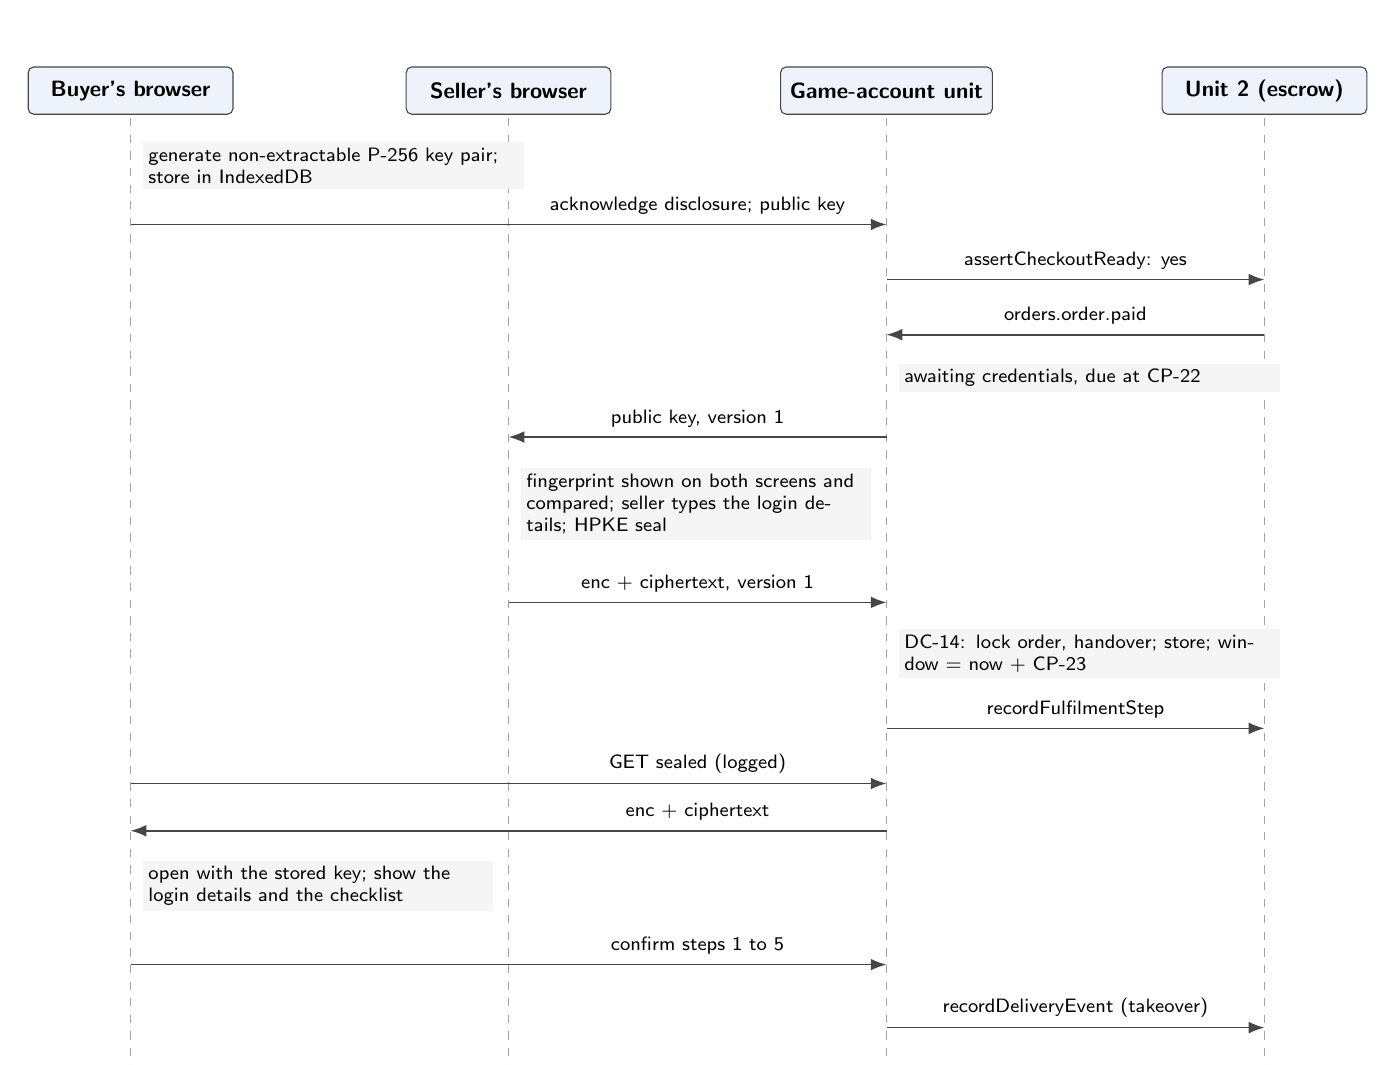
\begin{tikzpicture}[font=\sffamily\footnotesize,
  actor/.style={draw=edge, fill=boxb, rounded corners=2pt, minimum width=2.6cm, minimum height=0.6cm, font=\sffamily\footnotesize\bfseries},
  msg/.style={-{Latex[length=2mm]}, draw=edge, semithick},
  note/.style={font=\sffamily\scriptsize, align=left, text width=4.7cm, anchor=west, fill=boxd, inner sep=2pt}]
\def\B{0} \def\S{4.8} \def\A{9.6} \def\E{14.4}
\foreach \x/\t in {\B/Buyer's browser, \S/Seller's browser, \A/Game-account unit, \E/Unit 2 (escrow)}{
  \node[actor] at (\x,0) {\t};
  \draw[edge!50, dashed] (\x,-0.35) -- (\x,-12.5);}
\node[note] at (\B+0.15,-0.95) {generate non-extractable P-256 key pair; store in IndexedDB};
\draw[msg] (\B,-1.7) -- node[above, font=\sffamily\scriptsize, pos=0.75]{acknowledge disclosure; public key} (\A,-1.7);
\draw[msg] (\A,-2.4) -- node[above, font=\sffamily\scriptsize]{assertCheckoutReady: yes} (\E,-2.4);
\draw[msg] (\E,-3.1) -- node[above, font=\sffamily\scriptsize]{orders.order.paid} (\A,-3.1);
\node[note] at (\A+0.15,-3.65) {awaiting credentials, due at CP-22};
\draw[msg] (\A,-4.4) -- node[above, font=\sffamily\scriptsize]{public key, version 1} (\S,-4.4);
\node[note, text width=4.3cm] at (\S+0.15,-5.25) {fingerprint shown on both screens and compared; seller types the login details; HPKE seal};
\draw[msg] (\S,-6.5) -- node[above, font=\sffamily\scriptsize]{enc + ciphertext, version 1} (\A,-6.5);
\node[note] at (\A+0.15,-7.15) {DC-14: lock order, handover; store; window = now + CP-23};
\draw[msg] (\A,-8.1) -- node[above, font=\sffamily\scriptsize]{recordFulfilmentStep} (\E,-8.1);
\draw[msg] (\B,-8.8) -- node[above, font=\sffamily\scriptsize, pos=0.75]{GET sealed (logged)} (\A,-8.8);
\draw[msg] (\A,-9.4) -- node[above, font=\sffamily\scriptsize, pos=0.25]{enc + ciphertext} (\B,-9.4);
\node[note, text width=4.3cm] at (\B+0.15,-10.1) {open with the stored key; show the login details and the checklist};
\draw[msg] (\B,-11.1) -- node[above, font=\sffamily\scriptsize, pos=0.75]{confirm steps 1 to 5} (\A,-11.1);
\draw[msg] (\A,-11.9) -- node[above, font=\sffamily\scriptsize]{recordDeliveryEvent (takeover)} (\E,-11.9);
\end{tikzpicture}}
\caption{Sealed handover and takeover. Nothing to the right of the browsers can read the login details.}
\label{fig:seq}
\end{figure}

\begin{itemize}[nosep]
  \item \textbf{When.} The seller is asked for the credentials only after payment is \texttt{held}, and must deliver them by CP-22 (24~hours after payment); otherwise Unit~2 refunds the buyer in full (FR-GAM-10). The database refuses a delivery at or after that deadline.
  \item \textbf{What.} The seller's screen has fields for the login identifier, the password, recovery codes and a note. The fields have spell-checking and autocomplete turned off, because some browsers send spell-checked text to an online service. The values are serialised to JSON, prefixed with their length and padded with zeros to a multiple of 512 bytes, at most 4~KB (DV-34). Padding hides the password's length: a 5-character and a 300-character password give ciphertexts of the same size (tested).
  \item \textbf{For which key.} The ciphertext names the key version it was sealed for. The database refuses a version that is not the buyer's current one, so a seller who sealed for the old key after a re-key is told to seal again.
  \item \textbf{Exactly once.} A second delivery for the same key is refused. Ten simultaneous deliveries produced one ciphertext. The first delivery is reported to Unit~2 as the fulfilment step.
\end{itemize}

\subsection{Retrieval and the access log}
Only the buyer of the order, from an authenticated session, can retrieve the ciphertext (FR-GAM-11). Every retrieval writes a row to the append-only access log: order, user, session, key version, source address and time (SEC-GAM-02). Twenty simultaneous retrievals produced twenty log rows. The log is kept for 2~years after the order closes (SRS retention schedule). The opened credentials exist only in the page: the view hides them after DV-38 (2~minutes) without activity, and the copy button clears the clipboard after 60~seconds where the browser allows.

\subsection{Re-key}
\label{sec:rekey}
A buyer who loses the private key, for example by clearing browser data or changing device, can ask for one re-key during the takeover window (FR-GAM-12):
\begin{enumerate}[nosep]
  \item the new browser generates a new key pair (version 2) and sends its public key;
  \item the takeover window stops; the old ciphertext stays readable but is useless to the buyer;
  \item the seller is asked to seal again for version 2, by DV-37 (CP-22, 24~hours, after the request);
  \item the new delivery deletes the old ciphertext and starts a new full takeover window. It is not a second fulfilment step for Unit~2.
\end{enumerate}
A re-key is refused once the buyer has confirmed changing the recovery e-mail: by then the buyer controls the account and needs no credentials. Only one re-key is allowed; ten simultaneous requests produced one new key. If the seller does not seal again in time, the handover becomes \texttt{disputed}, and Unit~7 opens a \texttt{credentials\_invalid} dispute on the buyer's behalf, because the buyer can no longer get in through no fault of the platform's rules.

% ------------------------------------------------------------------
\section{Takeover and Protection}
\label{sec:takeover}

\subsection{The checklist}
When the buyer opens the credentials, the screen shows the takeover checklist with a countdown of the window and the date on which the protection period will end (FR-GAM-13, NFR-USE-03):
\begin{enumerate}[nosep]
  \item change the password;
  \item change the recovery e-mail;
  \item change the recovery phone;
  \item remove linked social logins;
  \item turn on two-step verification.
\end{enumerate}
Each step is confirmed by the buyer and stored once, with its session and time, in the append-only \texttt{confirmations} table. A confirmed step can never be undone.

\subsection{Completion}
The takeover is complete, and the order's delivery event happens, at the first of:
\begin{itemize}[nosep]
  \item the buyer's confirmation of the fifth step; ten simultaneous confirmations of the last step produced one completion and one event;
  \item the end of the takeover window CP-23 (24~hours after delivery), if the buyer has neither finished nor reported a problem (FR-GAM-15). The completion time recorded is the end of the window, not the time the job happened to run, so the protection period is not lengthened by job delay.
\end{itemize}
On completion the service calls \texttt{recordDeliveryEvent(game\_takeover, at)} in the same DC-14 transaction. Unit~2 then holds the payment until \texttt{at} $+$ CP-24 (7~days), under its \texttt{game\_protection} release policy, and the general auto-release CP-19 does not apply (FR-GAM-16, FR-GAM-17).

\begin{figure}[!htbp]
\centering
\resizebox{\textwidth}{!}{%
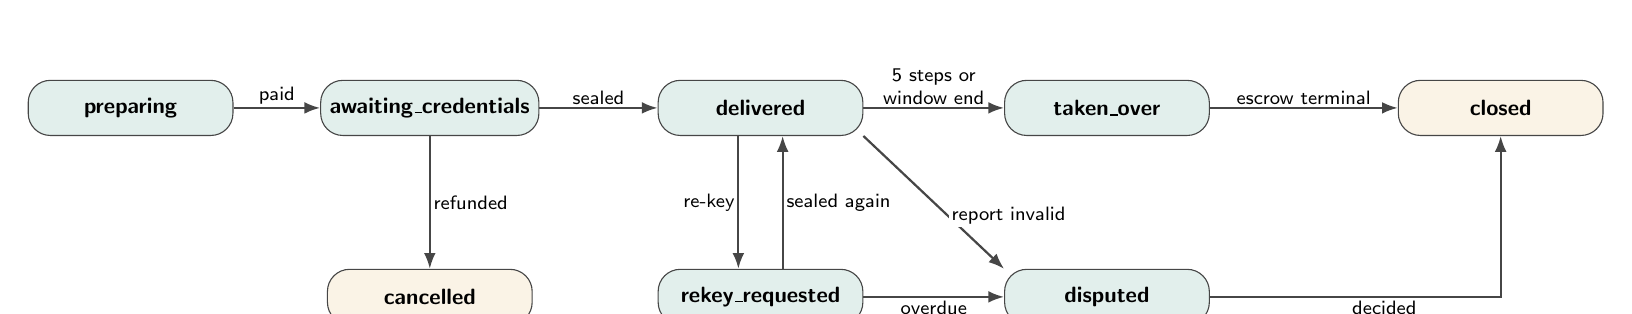
\begin{tikzpicture}[font=\sffamily\footnotesize,
  st/.style={draw=edge, rounded corners=8pt, fill=boxa, minimum width=2.6cm, minimum height=0.7cm, font=\sffamily\footnotesize\bfseries},
  tst/.style={st, fill=boxc},
  tr/.style={-{Latex[length=2mm]}, draw=edge, thick},
  lb/.style={font=\sffamily\scriptsize, align=center, fill=white, inner sep=1pt}]
\node[st] (p) at (0,0) {preparing};
\node[st] (a) at (3.8,0) {awaiting\_credentials};
\node[st] (d) at (8.0,0) {delivered};
\node[st] (t) at (12.4,0) {taken\_over};
\node[tst] (cl) at (17.4,0) {closed};
\node[st] (r) at (8.0,-2.4) {rekey\_requested};
\node[st] (x) at (12.4,-2.4) {disputed};
\node[tst] (cn) at (3.8,-2.4) {cancelled};
\draw[tr] (p) -- node[lb, above]{paid} (a);
\draw[tr] (a) -- node[lb, above]{sealed} (d);
\draw[tr] (d) -- node[lb, above, align=center]{5 steps or\\window end} (t);
\draw[tr] (t) -- node[lb, above]{escrow terminal} (cl);
\draw[tr] ([xshift=-8pt]d.south) -- node[lb, left]{re-key} ([xshift=-8pt]r.north);
\draw[tr] ([xshift=8pt]r.north) -- node[lb, right]{sealed again} ([xshift=8pt]d.south);
\draw[tr] (d.south east) -- node[lb, right, pos=0.6]{report invalid} (x.north west);
\draw[tr] (r) -- node[lb, below]{overdue} (x);
\draw[tr] (x.east) -| node[lb, below, pos=0.3]{decided} (cl.south);
\draw[tr] (a) -- node[lb, right]{refunded} (cn);
\end{tikzpicture}}
\caption{Handover status. Terminal states are shaded. Not drawn: \texttt{preparing}, \texttt{delivered} and \texttt{rekey\_requested} also go to \texttt{cancelled} on a refund before the delivery event, and a withdrawn dispute returns to \texttt{delivered}. The trigger \texttt{handover\_guard} refuses every other change.}
\label{fig:states}
\end{figure}

\subsection{``The credentials do not work''}
Within the takeover window, the buyer may report that the credentials do not work (FR-GAM-14). The service marks the handover \texttt{disputed} and opens a \texttt{credentials\_invalid} dispute in Unit~7 in the same transaction; the window then no longer runs, so the takeover cannot complete while the dispute is open. The report is refused once the buyer has confirmed changing the recovery e-mail, because a buyer who could change it clearly got in. This is the one race in the unit where a person can act against themselves, so it was tested directly: on 20 orders, a report and the recovery-e-mail confirmation were submitted at the same moment. On every order exactly one of them succeeded, never both (three runs; the split between them varied). If the buyer withdraws the dispute, the takeover resumes, and if its window has meanwhile ended, the next job run completes it.

\subsection{Protection period and seller recovery}
During the protection period the buyer can open a \texttt{seller\_recovery} dispute with evidence such as the publisher's security e-mails (FR-GAM-16). The buyer can also release the payment early, with step-up authentication, through Unit~2 (FR-GAM-17, SEC-AUTH-08).

\label{sec:evidence}
When an operator confirms that a seller recovered a sold account, during the protection period or by a report after release, Unit~7 suspends the seller and adds the seller's NID blind index to the blacklist with four-eyes approval, through Unit~1 (FR-GAM-18). For the complaint to law enforcement, \texttt{GameAccountQueries.evidence} supplies:
\begin{itemize}[nosep]
  \item the listing details, the ownership code and the operator's review, with a signed link to the screenshot;
  \item the timeline: payment, credential deliveries with key versions, re-key, each confirmed step with its session, and the takeover;
  \item the credential-access log;
  \item the fingerprints of the buyer's keys, which show which key each delivery was sealed for.
\end{itemize}
The evidence contains no ciphertext and no public key. The ciphertext would be useless to anyone but the buyer, and by then it has usually been deleted.

\subsection{Deletion}
When the order's escrow reaches a terminal state and no dispute is open, the ciphertext is deleted: its bytes are removed and only the deletion time is kept (FR-GAM-19). A refund before the takeover deletes it too. The database refuses to close or cancel a handover while any ciphertext remains, and the only change ever allowed to a sealed-credentials row is this deletion. The public keys, access log and confirmations stay, as evidence (SRS retention schedule).
\section{Scheduled Jobs}
\label{sec:jobs}
Each job scans due rows through a partial index and is safe on several instances (\texttt{FOR UPDATE SKIP LOCKED}). The deadline refunds themselves are Unit~2's jobs.
\begin{dtable}{@{}>{\raggedright\arraybackslash}p{3.6cm}>{\raggedright\arraybackslash}p{1.8cm}>{\raggedright\arraybackslash}p{9.8cm}@{}}
\toprule
\textbf{Job} & \textbf{Every} & \textbf{Action} \\ \midrule \endhead
Takeover window end & 1 min & \texttt{complete\_if\_due}: complete takeovers whose window has ended, at the end time, and record the delivery event (FR-GAM-15). \\
Re-key overdue & 5 min & \texttt{rekey\_overdue}: move unanswered re-keys to \texttt{disputed} and open the dispute (DV-37). \\
Proof expiry & 1 hour & Mark issued codes past DV-33 as \texttt{expired}. \\
\bottomrule
\end{dtable}
The window-end job compares with the statement clock (\texttt{clock\_timestamp()}) rather than the transaction start, so a job transaction that began a moment before the deadline still sees it pass.

\section{Security}

\subsection{Controls}
\begin{itemize}[nosep]
  \item \textbf{No readable credentials on the server} (SEC-GAM-01). The private key is generated non-extractable in the buyer's browser and never leaves it; the server stores only public keys, \texttt{enc} and ciphertexts. No server code path has a decryption key, and no staff endpoint returns a ciphertext.
  \item \textbf{Standard cryptography only} (SEC-DAT-10, C-4): HPKE (RFC~9180) with DHKEM(P-256, HKDF-SHA256), HKDF-SHA256 and AES-256-GCM, through a library built on the Web Cryptography API. The team writes no primitive and no construction.
  \item \textbf{Binding.} Associated data ties each ciphertext to its order and key version; the database ties each ciphertext to an existing key version, and refuses any length that is not padded.
  \item \textbf{Strict pages} (SEC-GAM-03). The credential-entry and credential-view routes load no third-party script, with a nonce-based Content Security Policy and \texttt{script-src 'self'} only; no analytics, error-reporting or chat widget is loaded on them. Responses are \texttt{no-store}. The fields have autocomplete and spell-checking off.
  \item \textbf{Nothing secret elsewhere} (SEC-DAT-07, FR-NTF-08). Ciphertext, keys and the plaintext never appear in logs, analytics, URLs, notifications or event payloads. Request logging for the sealed endpoints records the size only.
  \item \textbf{Integrity and evidence.} Public keys, the access log and the confirmations are append-only; a sealed-credentials row can only be emptied. The application role cannot update these tables or delete sealed rows (tested).
\end{itemize}

\subsection{Threats considered}
\begin{dtable}{@{}>{\raggedright\arraybackslash}p{4.6cm}>{\raggedright\arraybackslash}p{10.6cm}@{}}
\toprule
\textbf{Threat} & \textbf{Defence, or limit} \\ \midrule \endhead
Database or backup stolen & Only public keys and ciphertexts: nothing decryptable. \\
Operator curious or bribed & No endpoint returns ciphertext; it is useless without the buyer's browser anyway; screenshot views audited. \\
Server swaps the buyer's key & Fingerprints computed in both browsers and compared, ideally by phone. Limit: a fully compromised server could also alter the code it sends (AS-6); reduced by the change controls of SEC-SDL. \\
Ciphertext moved to another order & Associated data: fails to open (tested). \\
Seller lists an account he does not control & Fresh code on the live profile; screenshot alone not enough when the profile is public. \\
Someone blocks another's player ID & Claims are taken only on approval, not on drafting. \\
Seller recovers the account after sale & Payment held for CP-24 after takeover; \texttt{seller\_recovery} dispute; suspension, blacklist and evidence (FR-GAM-18). \\
Buyer falsely says ``they do not work'' & Refused once the recovery-e-mail step is confirmed; the access log shows every retrieval and the confirmations show what the buyer did. \\
Publisher bans the account & Not preventable; disclosed and acknowledged before payment (FR-GAM-05). \\
Malicious browser extension on a user's device & Out of scope: the SRS excludes compromise of a user's own device; the buyer is advised to use a clean browser profile. \\
\bottomrule
\end{dtable}

\section{Parameters}
\textbf{SRS parameters used:} CP-22 (credential delivery); CP-23 (takeover window); CP-24 (protection period, applied by Unit~2); CP-31 (signed links); CP-33 (upload size); CP-36 (feature switch).

\textbf{Design values introduced} (continuing DV-1 to DV-32):
\begin{dtable}{@{}>{\bfseries}p{1.3cm}>{\raggedright\arraybackslash}p{4.4cm}>{\raggedright\arraybackslash}p{4.6cm}>{\raggedright\arraybackslash}p{4.6cm}@{}}
\toprule
\textnormal{\textbf{ID}} & \textbf{Value} & \textbf{Default} & \textbf{Reason} \\ \midrule \endhead
DV-33 & Ownership code & \texttt{TB-XXXX-XXXX}, 40 random bits (Crockford base32); valid 7 days & Fresh, easy to type into a profile. \\
DV-34 & Sealed payload & length prefix, JSON, zero-padded to 512-byte blocks; at most 4 KB & Hides password length; bounds storage. \\
DV-35 & HPKE suite and context & base mode; DHKEM(P-256, HKDF-SHA256), HKDF-SHA256, AES-256-GCM; info \texttt{TrustBazaar/\allowbreak game-credentials/\allowbreak v1}; AAD \texttt{order:<id>|\allowbreak key:<v>} & SEC-DAT-10's ECDH option in its standard form. \\
DV-36 & Key fingerprint & first 80 bits of SHA-256 of the raw key; 5 groups of 4 hex digits & Short enough to read out; too long to forge. \\
DV-37 & Re-delivery after a re-key & CP-22 after the request; then a dispute & Same time as the first delivery. \\
DV-38 & Credential view & hidden after 2 min idle; clipboard cleared after 60 s & Shortens exposure on a shared screen. \\
DV-39 & Ownership screenshot retention & 2 years after the last order on the listing closes; 30 days after a rejection or an unsold end & Evidence for FR-GAM-18; not in the SRS schedule (I-35). \\
\bottomrule
\end{dtable}

\section{Testing}
\label{sec:testing}
\begin{dtable}{@{}>{\raggedright\arraybackslash}p{3.2cm}>{\raggedright\arraybackslash}p{12cm}@{}}
\toprule
\textbf{Level} & \textbf{Cases} \\ \midrule \endhead
Database (done) & 70 checks in \texttt{05\_game\_accounts\_tests.sql}, each rejection required to fail on its intended rule: game details and platform; ownership codes, proof submission and review, live-profile and expiry rules, claims; disclosure, key format and fixing; the fingerprint vector; delivery before payment, by the wrong party, for the wrong key, unpadded, too long, after the deadline, twice; retrieval and its log; checklist steps, undoing, completion by checklist and by window end; reports before and after the recovery-e-mail step; withdrawal; re-key, re-delivery and overdue; deletion, closing and cancelling; events and grants. The Unit~1 to~4 scripts still pass with this schema loaded. \\
Concurrency (done) & Six races, three runs each on fresh databases (Appendix~\ref{app:tests}): 10 approvals of one player ID (1 approved); 10 deliveries (1 ciphertext); 10 final steps (1 completion); 10 re-keys (1 new key); 20 retrievals (20 log rows); on 20 orders a report against the recovery-e-mail step (never both). \\
Browser (done) & 14 checks of \texttt{sealed.js} in real Chromium through Playwright: the private key is non-extractable and survives a reload in IndexedDB; buyer and seller compute the same fingerprint; ciphertext sizes; the password is absent from the ciphertext; tampering, another order, another key version and another key all fail; over-long input is refused; lengths are hidden; each seal uses a fresh \texttt{enc}; the fingerprint vector matches the database. The browser's real ciphertext was then accepted by \texttt{game\_accounts.deliver}. \\
Planned & Firefox and Safari runs of the browser test (Playwright WebKit and Firefox); the RFC~9180 test vectors for DHKEM(P-256, HKDF-SHA256) through the library; negative authorisation tests for every endpoint (SEC-SDL-09); a CSP test that the credential pages load no third-party origin; a log scan in CI for ciphertext and key material. \\
\bottomrule
\end{dtable}

\section{Notes for Integration}
\label{sec:notes}
\begin{enumerate}[label=\textbf{I-\arabic*}, leftmargin=*, nosep]
  \setcounter{enumi}{28}
  \item \textbf{Unit 2.} \texttt{GameAccountPort.assertCheckoutReady} is \texttt{checkout\_ready} plus the CP-36 check. \texttt{orders.order.paid} for a game account must carry \texttt{fulfilment\_due\_at} (CP-22), as I-19 already requires. The first delivery calls \texttt{recordFulfilmentStep(credentials\_delivered)}; completion calls \texttt{recordDeliveryEvent(game\_takeover, at)} with the recorded completion time, which may be slightly in the past. Escrow-terminal events must say whether the delivery event had happened.
  \item \textbf{Unit 3.} Publish \texttt{listings.listing.cancelled} as well, so a claim can be released. While CP-36 is off, refuse game-account publishing and purchases, and leave game-account listings out of \texttt{listings.searchable}. Add password words in Bangla and English to the screening terms.
  \item \textbf{Unit 1.} \texttt{FileVault} gains a purpose for ownership screenshots, on its own volume, with retention DV-39. The CP-36 switch is one of the administrator controls under four-eyes approval (SEC-IRM-04). Suspension and blacklisting for FR-GAM-18 use the existing approvals.
  \item \textbf{Unit 6.} Notify the seller when credentials are requested and the buyer when they are delivered, and remind both at CP-38 before the credential deadline, the window end and the protection end (FR-NTF-07). No notification contains credentials, keys or fingerprints. For FR-GAM-20 (Could), warn a seller whose chat message looks like login details (for example ``password'' or ``pass'' in Bangla or English next to a token, or an e-mail address with another string) and link to the sealed handover. The warning never blocks or stores the message's content.
  \item \textbf{Unit 7.} The ownership-proof queue (FR-OPS-01) calls \texttt{reviewProof}. A \texttt{credentials\_\allowbreak invalid} dispute is opened in the same transaction as the report, and also when a re-key is overdue. A withdrawal calls \texttt{disputeWithdrawn}. The case file and the FR-GAM-18 export use \texttt{evidence}.
  \item \textbf{Unit 8.} Screens of IF-UI-06 use \texttt{sealed.js}; check Web Crypto and IndexedDB before purchase (AS-5); warn the buyer to stay in the same browser; follow the strict-page rules of the security section. The browser module needs \texttt{@hpke/core} pinned to an exact version and bundled into the application, not loaded from a CDN, because a CDN would be a third-party script on the credential pages (SEC-GAM-03).
  \item \textbf{SRS clarifications proposed:}
  \begin{itemize}[nosep]
    \item SEC-DAT-10: name HPKE (RFC~9180) with the suite of DV-35 as the form of the ECDH option, and note the 318-byte limit of RSA-OAEP-3072;
    \item FR-GAM-12: a re-key is not possible after the recovery-e-mail step, and the seller must seal again within CP-22, or a dispute is opened;
    \item FR-GAM-15: at the window end the completion time is the end of the window;
    \item retention schedule: add ownership screenshots (DV-39);
    \item add DV-33 to DV-39 to the SRS parameter table.
  \end{itemize}
\end{enumerate}

\appendix
\section{Traceability}
\label{app:trace}
{\small\begin{longtable}{@{}>{\ttfamily}p{2.4cm}>{\raggedright\arraybackslash}p{10.6cm}>{\raggedright\arraybackslash}p{2.2cm}@{}}
\toprule \textnormal{\textbf{Requirement}} & \textbf{Design element} & \textbf{Section} \\ \midrule \endhead
FR-GAM-01 & CP-36 checked at listing and checkout; hidden listings; paid orders continue & \ref{sec:listing} \\
FR-GAM-02 & \texttt{details}; no login fields; screening terms & \ref{sec:listing} \\
FR-GAM-03 & Ownership codes; encrypted screenshot; live-profile check; \texttt{review\_proof} & \ref{sec:review} \\
FR-GAM-04 & \texttt{claims}, unique while live, taken on approval, released at escrow end & \ref{sec:review} \\
FR-GAM-05 & Disclosure version and acknowledgement; \texttt{checkout\_ready} & \ref{sec:sealed} \\
FR-GAM-06 & No delivery unit; Unit~2 constraints & \ref{sec:data} \\
FR-GAM-07 & Non-extractable P-256 key in IndexedDB; public key only to the server & \ref{sec:sealed} \\
FR-GAM-08 & Fingerprint computed in both browsers, never by the server & \ref{sec:fingerprint} \\
FR-GAM-09 & HPKE seal in the seller's browser; padding & \ref{sec:sealed} \\
FR-GAM-10 & Request after payment; delivery refused after CP-22 & \ref{sec:sealed} \\
FR-GAM-11 & \texttt{fetch\_sealed}: buyer only; append-only access log & \ref{sec:sealed} \\
FR-GAM-12 & One re-key; window restarts; DV-37 & \ref{sec:rekey} \\
FR-GAM-13 & Checklist; confirmations; countdown & \ref{sec:takeover} \\
FR-GAM-14 & \texttt{report\_invalid}; refused after the recovery-e-mail step & \ref{sec:takeover} \\
FR-GAM-15 & Completion by five steps or window end; delivery event & \ref{sec:takeover} \\
FR-GAM-16 & Protection period held by Unit~2; \texttt{seller\_recovery} disputes & \ref{sec:takeover} \\
FR-GAM-17 & Release at protection end or early with step-up (Unit~2) & \ref{sec:takeover} \\
FR-GAM-18 & Evidence; suspension and blacklist through Units~7 and~1 & \ref{sec:evidence} \\
FR-GAM-19 & Ciphertext deleted at the end; trigger refuses closing otherwise & \ref{sec:takeover} \\
FR-GAM-20 & Chat warning (Unit~6) & \ref{sec:notes} \\
FR-DSP-05 & \texttt{evidence}: proof, access log, confirmations & \ref{sec:evidence} \\
FR-NTF-08 & No secrets in notifications or events & \ref{sec:api} \\
SEC-GAM-01 & Trust boundary; no decryption key on the server & \ref{sec:boundary} \\
SEC-GAM-02 & Append-only access log & \ref{sec:sealed} \\
SEC-GAM-03 & Strict pages, no third-party scripts, bundled library & \ref{sec:notes} \\
SEC-DAT-07 & Nothing secret in logs, URLs or analytics & \ref{sec:notes} \\
SEC-DAT-10 & HPKE with P-256 and AES-256-GCM & \ref{sec:sealed} \\
IF-UI-06 & Screens and their rules & \ref{sec:notes} \\
IF-SW-07 & Web Cryptography API through \texttt{@hpke/core} & \ref{sec:sealed} \\
NFR-USE-03 & Countdown and protection end on the checklist & \ref{sec:takeover} \\
NFR-MNT-02 & Release-rule, race and browser tests & \ref{sec:testing} \\
DR-07 & Details, proofs, keys, ciphertext until deletion, confirmations, access log & \ref{sec:data} \\
\bottomrule
\end{longtable}}

\section{Database Schema and Tests}
\label{app:ddl}
\subsection{Test results}
\label{app:tests}
Loaded after the Unit~1 to Unit~4 schemas in PostgreSQL 16, using PostgreSQL 15 features only. Every check passed.
{\scriptsize
\begin{verbatim}
PASS  FR-GAM-02 the platform must be one the game offers [is not offered for this game]
PASS  player IDs are compared without spaces and case
PASS  DV-33 ownership codes have the fixed format [ownership_proofs_code_check]
PASS  one open ownership proof per listing [proof_one_open]
PASS  a proof cannot be reviewed before the screenshot is submitted [not awaiting review]
PASS  submitting needs the screenshot [proof_submitted_fields]
PASS  the game and player ID are fixed once proof is submitted [fixed once ownership proof]
PASS  an operator cannot approve a proof whose live profile did not match [proof_approve_live]
PASS  FR-GAM-03 a rejection needs a reason [proof_reject_reason]
PASS  FR-GAM-03 approval records the operator and takes the player-ID claim
PASS  ... claim and event written
PASS  a reviewed proof is final [reviewed proof is final]
PASS  FR-GAM-04 one live listing per game and player ID: the second approval is refused [already listed]
PASS  DV-33 an expired code cannot be approved [has expired]
PASS  FR-GAM-07 no key before the disclosure is acknowledged [acknowledge the disclosure first]
PASS  a handover starts as preparing, without a key [starts as preparing]
PASS  FR-GAM-05 with the disclosure acknowledged but no key, checkout is not ready
PASS  FR-GAM-07 a public key must be an uncompressed P-256 point [buyer_keys_public_key_check]
PASS  only the buyer registers a key [only the buyer]
PASS  FR-GAM-07 key version 1 registered; checkout is ready
PASS  ... ready
PASS  the key cannot be swapped once registered [key is fixed at checkout]
PASS  buyer keys are append-only [append-only]
PASS  FR-GAM-08 fingerprint test vector (first 80 bits of SHA-256 of the raw key)
PASS  FR-GAM-10 credentials are not accepted before payment [not expected now]
PASS  only the seller delivers [only the seller]
PASS  ciphertext must be sealed for the buyer's current key [current key is version 1]
PASS  DV-34 an unpadded ciphertext length is refused [sealed_credentials_ciphertext_check]
PASS  DV-34 the payload is at most 4 KB [sealed_credentials_ciphertext_check]
PASS  the encapsulated key must be a P-256 point [sealed_credentials_enc_check]
PASS  FR-GAM-09 the first delivery is the fulfilment step and starts the CP-23 window
PASS  ... window ends 24 hours after delivery
PASS  credentials are delivered once (no second ciphertext without a re-key) [not expected now]
PASS  sealed credentials cannot be altered, only deleted [can only be deleted]
PASS  FR-GAM-10 nothing is accepted after the CP-22 deadline [deadline has passed]
PASS  FR-GAM-11 only the buyer of the order can retrieve the ciphertext [only the buyer]
PASS  FR-GAM-11 every retrieval is logged with user, session and time
PASS  SEC-GAM-02 the access log is append-only [append-only]
PASS  only the buyer confirms takeover steps [only the buyer]
PASS  FR-GAM-13 confirming the password step does not complete the takeover
PASS  FR-GAM-14 after the recovery e-mail step, credentials_invalid is refused [no longer accepted]
PASS  FR-GAM-12 no re-key after the recovery e-mail step [already controls the recovery e-mail]
PASS  a step confirmed twice is recorded once
PASS  a confirmed step cannot be undone [fixed once recorded]
PASS  FR-GAM-15 the fifth step completes the takeover (the delivery event), source checklist
PASS  a completed takeover cannot be cancelled [is not permitted]
PASS  before the window ends, the job does nothing
PASS  FR-GAM-15 at the window end the takeover is treated as complete, at the end time
PASS  FR-GAM-14 a credentials_invalid report inside the window opens the dispute path
PASS  while disputed, no step can be confirmed [not in progress]
PASS  while disputed, the window-end job cannot complete the takeover
PASS  FR-DSP-10 a withdrawn dispute resumes the takeover window
PASS  a checklist completion needs all five confirmations [checklist_complete]
PASS  FR-GAM-12 a re-key issues key version 2 and stops the window
PASS  ... status rekey_requested, no window, re-delivery deadline set
PASS  the seller must seal for the new key, not the old one [current key is version 2]
PASS  FR-GAM-12 re-delivery restarts the window and is not a second fulfilment step
PASS  the old ciphertext is deleted on re-delivery; only version 2 can be retrieved
PASS  FR-GAM-12 only one re-key per order [one re-key has been used]
PASS  DV-37 a re-key the seller does not answer in time becomes a dispute
PASS  ... status disputed
PASS  FR-GAM-19 at the terminal escrow state the ciphertext is deleted and the access log kept
PASS  FR-GAM-04 after the protection period the player ID can be listed again
PASS  after closing, nothing can be retrieved [no credentials are available]
PASS  a closed handover is final [handover is closed]
PASS  FR-GAM-19 a handover cannot be closed while ciphertext remains [ciphertext must be deleted]
PASS  an order refunded before the takeover cancels the handover
PASS  DC-6 outbox events are named game_accounts.<entity>.<past> [outbox_event_type_check]
PASS  application role cannot rewrite takeover confirmations [permission denied]
PASS  application role cannot delete sealed credentials rows (only blank them) [permission denied]

70 checks passed (05_game_accounts_tests.sql, PostgreSQL 16.15 with the Unit 1-4 schemas loaded).
The Unit 1-4 test scripts still pass with Unit 5 loaded (46, 45, 67 and 93 checks).

Concurrency (05_game_accounts_concurrency.sh). Three runs on fresh databases; the first five
races gave the same counts each time; the split in the last race varies, but 'both' was always 0.
  1|
  1|
  1|
  1|
  1|
  1|
  1|
  1|
  1|
  1|
  1|
  1|
  1|
  1|
  1|
  1|
  1|
  1|
  1|
  1|
  1|
  1|
  1|
  1|
  1|
  1|
  1|
  1|
  1|
  1|
  t
  t
  t
  t
  t
  t
  t
  t
  t
  t
  t
  t
  t
  t
  t
  t
  t
  t
  t
  t
  t
  t
  t
  t
  t
  t
  t
  t
  t
  f
  f
  f
  f
  Approval race: 10 operators approve 10 listings of the same player ID at once
    results: approved 1, refused 9
    database: live claims for the player ID=1
  Delivery race: the seller's sealed credentials submitted 10 times at once
    results: accepted 1, refused 9
    database: ciphertexts=1
  Final-step race: the last checklist step confirmed 10 times at once
    results: completed 1, refused or no-op 9
    database: takeover events=1
  Re-key race: 10 re-key requests at once
    results: accepted 1, refused 9
    database: keys=2
  Retrieval storm: 20 retrievals at once
    results: returned 20
    database: access log rows=20
  Report-or-confirm race: 20 orders, each with an invalid-report and the e-mail step at once
    results: reports accepted 12, e-mail steps accepted 8
    database: disputed=12, e-mail confirmed=8, both=0

Browser (crypto/browser_test.mjs: sealed.js in real Chromium):
  PASS  FR-GAM-07 the private key is non-extractable
  PASS  FR-GAM-07 the public key is a 65-byte uncompressed P-256 point
  PASS  FR-GAM-08 buyer and seller compute the same fingerprint independently (eac3-2d92-149c-c061-d7e2)
  PASS  DV-34 ciphertext is 512 k + 16 bytes; enc is a 65-byte point (528 bytes)
  PASS  SEC-GAM-01 the ciphertext does not contain the password in clear
  PASS  FR-GAM-11 after a reload the stored key (still non-extractable) opens the credentials
  PASS  a modified ciphertext is rejected (AES-GCM tag)
  PASS  ciphertext moved to another order is rejected (associated data)
  PASS  ciphertext replayed under another key version is rejected
  PASS  another browser's key cannot open it
  PASS  DV-34 credentials over 4 KB are refused before sealing
  PASS  DV-34 a 5-character and a 300-character password give the same ciphertext size (528 bytes)
  PASS  each sealing uses a fresh encapsulated key
  PASS  FR-GAM-08 browser fingerprint of the test vector equals the SQL one (0ed3-a6ab-957f-f6f5-9a96)
  14 of 14 browser checks passed (Chromium via Playwright 1.56.0, @hpke/core 1.9.0)
  The browser's real ciphertext for the same key was then accepted by game_accounts.deliver.
\end{verbatim}
}
\subsection{Schema}
\lstinputlisting[language=SQLpg]{sql/05_game_accounts.sql}

\section{Browser Module}
\label{app:js}
The reference module \texttt{sealed.js}, as tested. Unit~8 imports it unchanged.
\lstinputlisting[language=JS]{crypto/sealed.js}
\end{document}
